\subsubsection{\stid{3.12} Sub-project: SUNDIALS}
\label{subsubsect:SUNDIALS-hypre}

\paragraph{Overview}

This project is enhancing the SUNDIALS library of numerical software packages for integrating differential systems in time using state-of-the-art time step technologies for use on exascale systems.

The SUNDIALS suite of packages \cite{SUNDIALSweb} provides efficient and adaptive time integrators and nonlinear solvers.  The packages are written using encapsulation of both data structures and solvers, thus allowing easy incorporation into existing codes and flexibility to take advantage of new solver technologies and packages.  SUNDIALS provides both multistep and multistage methods designed to evolve stiff or nonstiff ordinary (ODE) and differential algebraic (DAE) systems
with efficient accuracy-driven time step selection.
SUNDIALS also provides both Newton and fixed point (with optional acceleration) nonlinear solvers and scaled Krylov methods with hooks for user-supplied preconditioners.  Users can also supply their own nonlinear and linear solvers under the integrators.  SUNDIALS is released with data structures supporting several programming environments.  Users can employ these supplied structures or provide their own.

Through software infrastructure developments, this project is enabling the efficient and robust SUNDIALS time integrator packages to easily interoperate with applications evolving time dependent systems as well as with external linear and nonlinear solver packages developed for exascale computing.  In addition, this project is providing support for integrating several independent ordinary differential equation systems simultaneously on GPUs as part of multiphysics applications.  Lastly, this project is supporting the deployment and use of SUNDIALS packages within ECP applications, mainly through incorporation into the discretization-based Co-Design Centers, AMReX and CEED.

%% Efficient time integrators are essential for ECP because they are at the core of every time-dependent simulation application.  However, many applications do not use state-of-the-art methods, and if they do, they often do not yet use them fully on their systems.  For example, at the start of the ECP the astrophysics code, Nyx, used an adaptive integration package for solving individual reactions.  However, by applying a time integration package to a larger reaction system, the code is able to derive significant speedups through use of GPUs that execute more calculations concurrently thus getting an accurate solution much faster.  By allowing for solvers tuned to exascale systems and vectors that are heterogeneous, SUNDIALS will be more applicable for use in multiphysics systems running on exascale platforms.


\paragraph{Key Challenges}

Current implementations of efficient time integrators face challenges on many fronts.
First, applications need both efficient integrators and ones that can interface easily with efficient linear algebra
packages to solve subservient linear systems.  In addition, integrators and their interfaces to both solver libraries
and applications must be frequently updated to keep up with rapid advances in system architectures. Some ECP applications require the solution of many small systems of ODEs in parallel on GPUs giving rise to the need for
a GPU-enabled ODE integrator that can be used in parallel for many systems at once and be able to run on multiple GPU-based architectures with differing programming models. Lastly, ECP applications require assistance incorporating new linear solvers underneath the integrators and in updating their interfaces to optimally use integrators on new platforms.

%ODE integrators that can provide increasing functionalities, such as non-identity %mass matrices for solving systems of ODEs with finite element spatial %discretizations, and maintaining solutions on a constraint manifold.

\paragraph{Solution Strategy}

This project includes a number of implementation activities that will prepare the SUNDIALS suite of time integrators for systems found in ECP applications.  A major activity is developing support for evolving multiple systems of ODEs in parallel on AMD GPUs with the CVODE multistep
ODE integration package.  To meet this need, the SUNDIALS team has added support for assigning data structures and solvers to a particular GPU stream, thus making it possible for multiple instances of CVODE to simultaneously utilize the GPU in parallel.  CVODE has also been equipped with interfaces to a batched direct linear solver capable of using an NVIDIA  GPU.  Currently, new interfaces are being developed to provide these capabilities on AMD GPUs, as are expected for Frontier.  While these interfaces are straightforward for the vector operations, linear solvers that are AMD-GPU capable are not yet generally available.  SUNDIALS is working with ECP linear solver packages, such as Gingko and MAGMA, to take advantage of HIP-based solvers that they develop and that will be efficient for the expected systems.

In addition, this project is working to evaluate and optimize integrator performance within its ECP user applications.  A small test suite allowing easier evaluation of performance on new platforms is being developed.  This year, SUNDIALS will stand up this new test suite within the GitLab CI for testing from OLCF systems with the goal of using this infrastructure to evaluate performance.  Moreover, the SUNDIALS team is adding a performance assessment layer and enabling use of the ECP ST Caliper package for performance testing underneath that layer.  The SUNDIALS team plans to work with the AMPE phase field code (ExaAM project), PELEC, PELELM, and Nyx users to apply these tools in assessing and optimizing SUNDIALS' performance within their applications.

Lastly, the SUNDIALS team will provide general support to other ECP applications in interfacing SUNDIALS packages into their software and in the optimal use of advanced time integration algorithms.  This support will include working with the application teams to help them install SUNDIALS and adjust their build systems to appropriately link with the SUNDIALS library.

\paragraph{Recent Progress}
SUNDIALS had four releases this past year, including new features in direct support of ECP application needs.  In particular, releases in March and May 2020 included a new matrix implementation that interfaces to the sparse matrix implementation from the NVIDIA cuSparse library, new specialized fused CUDA kernels in CVODE which offer better performance on smaller problems when using CVODE with CUDA, new routines that support the ability to control kernel launch parameters for the CUDA vector and matrix modules, and new diagnostic routines that support load balancing efforts by making information on the difficulty of solves more accessible to users.  These features directly support capabilities needed in solving many small ODE systems simultaneously and have been integrated into the SUNDIALS use from AMReX-based applications, including Nyx, PELEC, and PELELM.

In addition, the May 2020 release also included new code to support integration of an ODE system while projecting onto a constraint manifold.  This capability, previously in a one-off package, CPODES, is needed by the AMPE phase field code in the ExaAM project.  The SUNDIALS team has worked with the AMPE team to incorporate the new version of CVODE into their software stack.

Lastly, the Sept. 2020 release included a new feature in the ARKODE package to support integration of systems with a time-dependent mass matrix.  This feature is needed by the MFEM high order discretization package in the CEED Co-Design center.

% In October of 2019, SUNDIALS 5.0.0 was released, including new vector structures that support flexible partitioning of solution data among different processing elements (e.g., CPU + GPU) or for multi-physics problems, an additional vector structure that supports MPI+X paradigms, and interfaces
% to high performance algebraic solver packages (SUPERLU\_DIST, the NVIDIA CUDA-based
% batched sparse QR direct linear solver, and the PETSc nonlinear solver SNES package).
% In September of 2019, the SUNDIALS team released a document quantifying performance of SUNDIALS codes on
% a demonstration problem that solves the three-dimensional nonlinear compressible Euler equations combined with advection and reaction of chemical species run using 40 cores on each of 2 to 3,456 nodes of the ORNL Summit machine.
% Figure \ref{fig:sun-many-demo} shows a diagram of the many-vector used in the demonstration problem where some solution components are distributed across the MPI processor decomposition and some are fully local.
% In addition to these activities, the SUNDIALS team has been collaborating closely with the AMReX Co-Design Center team to
% design effective interfaces to SUNDIALS time integrators from AMReX for applications using ODE integrators,
% such as for chemistry reaction systems as in Nyx, Castro, and PELE.  The PELELM and Nyx applications have both demonstrated use of the CVODE package from SUNDIALS within test runs utilizing new capabilities from SUNDIALS to run on Summit with GPUs.


%% In May of 2018, SUNDIALS 4.0.0-dev was released, including new fused vector kernels in the vector API and in all supplied vectors.  Results show speedup from using these routines, especially for parallel reductions.  In September of 2018, SUNDIALS 4.0.0-dev.2 was released, including a full redesign of the nonlinear solver interfaces to the time integrators and encapsulation of the nonlinear solevrs.  Figure \ref{fig:sunorg1} shows the new organization of SUNDIALS where separate nonlinear solver interfaces are provided for Newton and fixed point nonlinear solver methods.  These interfaces are shared across all SUNDIALS integrators.
%% Individual integrators have the freedom to supply specific information from the integrator that controls the solver.  In addition, the SUNDIALS team has been collaborating closely with the AMReX Co-Design Center team to
%% design effective interfaces to SUNDIALS time integrators from AMReX for applications using ODE integrators,
%% such as for chemistry reaction systems as in Nyx, Castro, and PELE.

\begin{figure}[htb]
	\centering
%	\includegraphics[width=6in]{projects/2.3.3-MathLibs/2.3.3.12-SUNDIALS-hypre/manyvector_v2.pdf}
	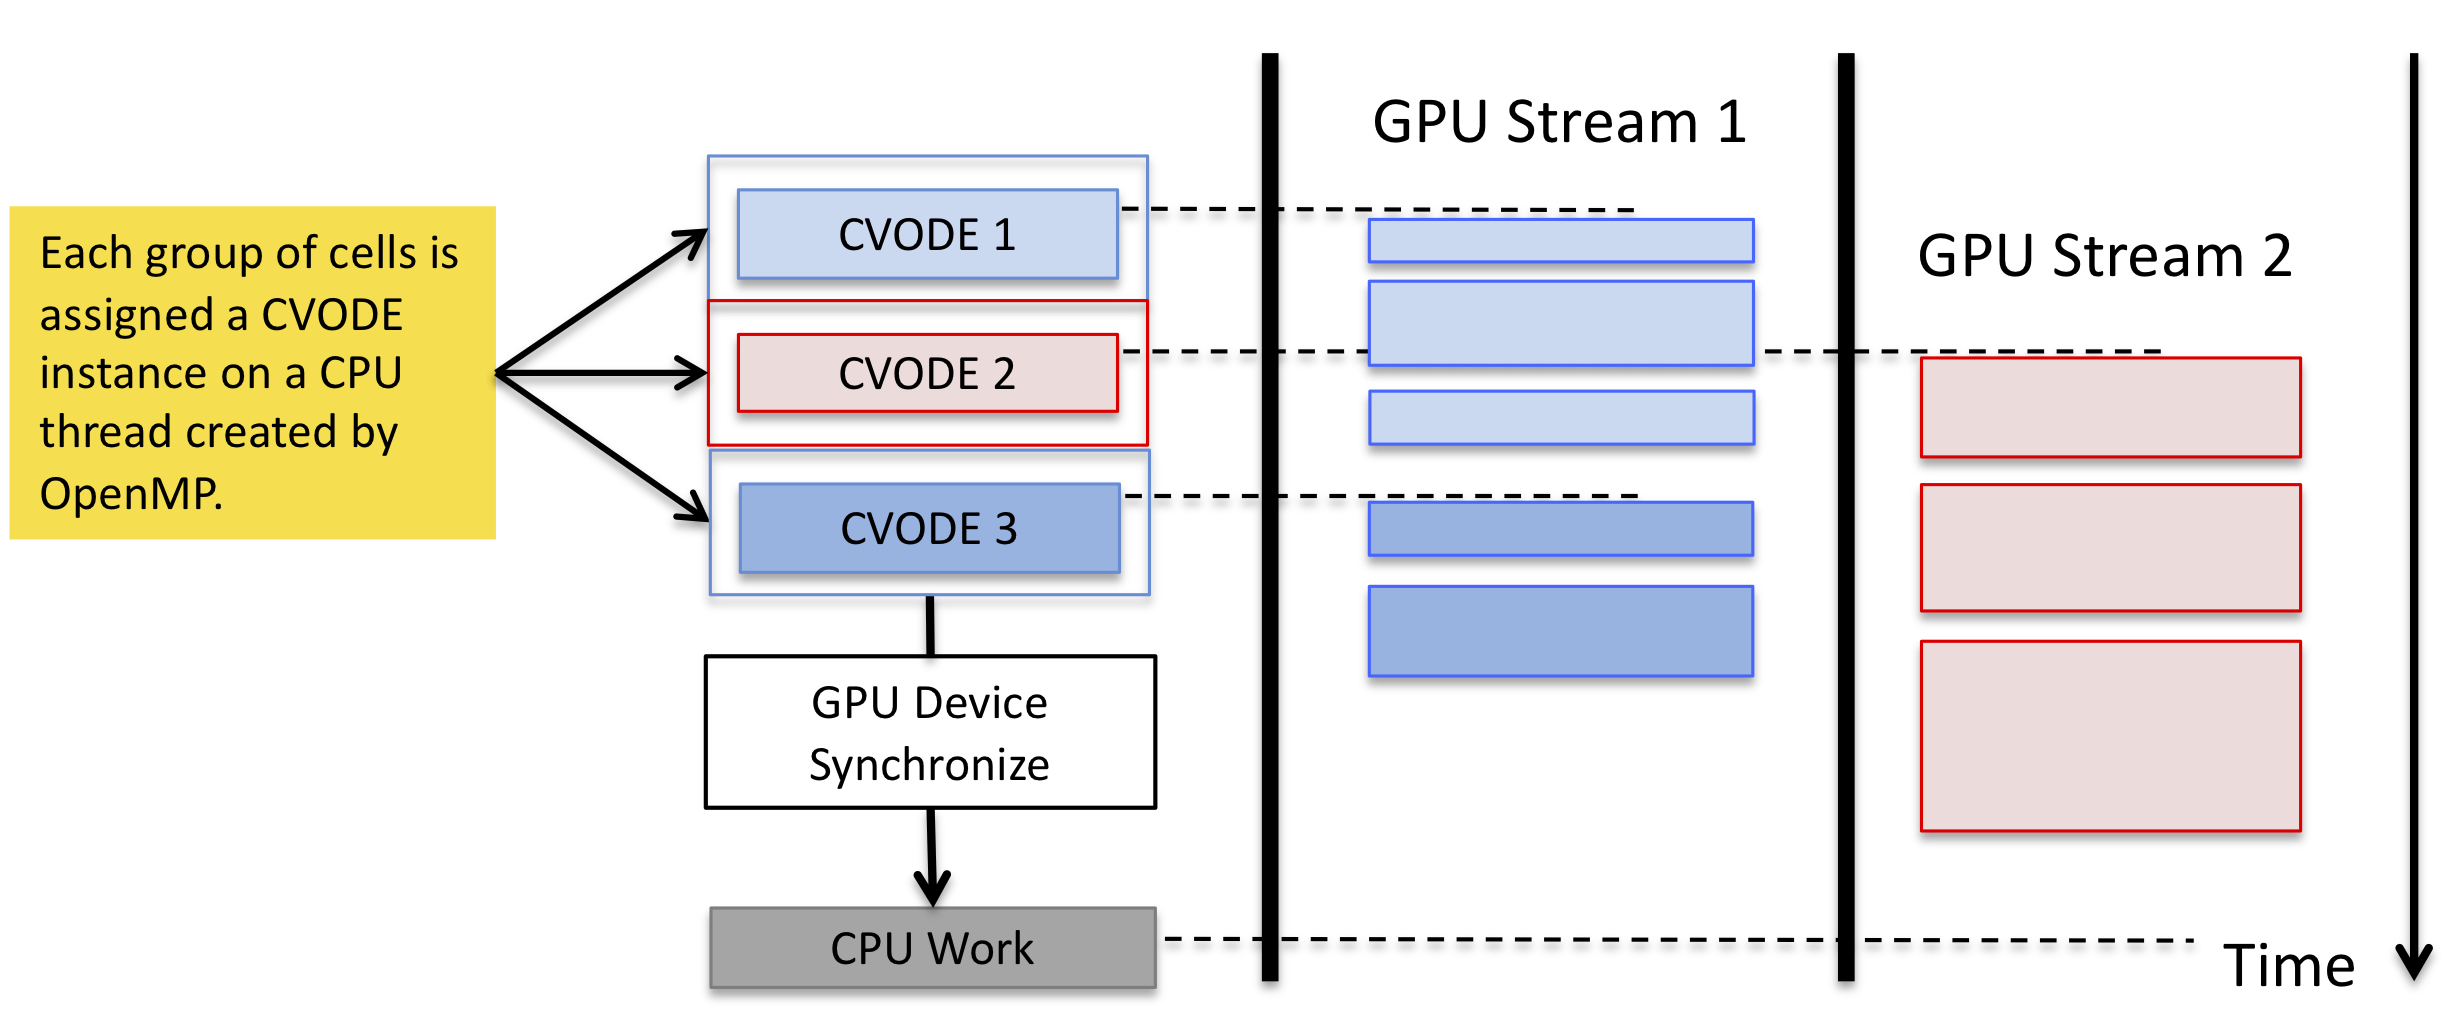
\includegraphics[width=0.9\linewidth]{projects/2.3.3-MathLibs/2.3.3.12-SUNDIALS-hypre/AMReX_CVODE_OpenMP_GPU-Streams-2.png}
	\caption{\label{fig:sun-many-demo} Illustration of SUNDIALS' hybrid, OpenMP + GPU approach to integrating the many small ODE systems that arise in the PELE and Nyx applications.  In this example, three distinct groups, formed by grouping the independent ODE systems arising in AMR grid cells, of ODE systems are integrated with CVODE. The groups, each defining a larger ODE system, are distributed across CPU threads with OpenMP. On each thread, a distinct and independent CVODE instance solves the larger ODE system. CVODE launches GPU kernels in streams, allowing some threads to operate simultaneously.}
\end{figure}




\paragraph{Next Steps}

During the remainder of FY21, this project team will:
\begin{enumerate}
\item Release SUNDIALS with vector and solver support for AMD GPUs.
\item Document performance of SUNDIALS within two ECP applications.
\item Expand SUNDIALS support for Intel GPUs.
\item Develop a performance test suite and document performance of SUNDIALS using GitLab and Caliper.
\item Continue to support AMReX and CEED Co-Design Centers in their use of SUNDIALS.
\end{enumerate}
